\documentclass[11pt,a4paper]{article}
\usepackage[T1]{fontenc}
\usepackage[utf8]{inputenc}
\usepackage{lmodern}
\usepackage[margin=2.5cm]{geometry}
\usepackage{graphicx}
\usepackage{hyperref}
\usepackage{booktabs}
\usepackage{xurl}
\usepackage{amsmath,amssymb}
\title{DenoiseOpt: Residual Scoring and Bi-Level Meta-Learning for Wavetable Wrap Crackle}
\author{Julian~M.~Kleber\\ORCID: \href{https://orcid.org/0000-0001-5518-0932}{0000-0001-5518-0932}\\Email: \href{mailto:julian.m.kleber@gmail.com}{julian.m.kleber@gmail.com}}
\date{18 July 2026 \\ \small Paper version \texttt{v3} (scientific writing workflow)}
\begin{document}
\maketitle
\begin{center}\small Code: \url{https://github.com/reeldemo/reelsynth}, \url{https://github.com/reeldemo/denoise-opt-meta}\end{center}
\begin{abstract}
Open wrap seams in periodic wavetable cycles inject audible crackle under cyclic playback. DenoiseOpt is a seam-local bake stack $f_\theta$, $\theta\in[0,1]^{12}$, scored without paired clean labels. We replace wrap-energy quality $Q$ as the outer meta objective with a prolonged residual score $R\in[0,1]$ (1~=~best): the engine's tiled DenoiseOpt cycle is compared to an ideal multi-period reference from the same seed with open-wrap cliffs withheld ($N{=}16$). The outer loop also nests an inner unsupervised loss fit $L=(1-\mathcal{D})+\lambda(1-\mathcal{S})$. Across 1500 literature-informed trials, Meta Top~1 \texttt{evo\_explore\_515} reaches residual $\approx 0.824$ vs naive DualCosine $\approx 0.698$ on held-out validation ($N{=}2000$)---a clear $+0.126$ margin---while keeping $\mathcal{S}\approx 1.0$. Nested loss-opt priors were searched but did not dominate the residual elite set; wide evolutionary mutation did.
\end{abstract}
\section{Introduction}
Wavetable synthesizers store one-period frames and wrap phase modulo one.
Discontinuous ends produce periodic broadband clicks. Classical DualCosine fades,
live BLEP, and related literature provide useful mechanisms
\cite{valimaki2006va,esqueda2016aliasing,esqueda2016blamp}, yet edited frames still
need a bake operator scored by prolonged playback agreement---not only a seam-local
proxy.

This paper separates \emph{seam-local} diagnostics from a \emph{prolonged}
evaluation score, and uses literature-informed search to select DenoiseOpt
parameters under that score.

Contributions:
\begin{enumerate}
  \item Define a prolonged residual score $R\in[0,1]$ against an ideal tiled reference ($N{=}16$).
  \item Nest an unsupervised loss fit inside literature-informed search priors while ranking by $R$.
  \item Report held-out evidence that \texttt{evo\_explore\_515} reaches residual $\approx 0.824$ versus DualCosine $\approx 0.698$ ($\Delta\approx +0.126$), with honest accounting that loss-opt elites lost to evolutionary explore.
\end{enumerate}

\section{Related Work}
We organize prior work by mechanism rather than by chronology. Domain-specific discontinuity control and virtual-analog anti-aliasing inform the operator design~\cite{valimaki2006va,esqueda2016aliasing,esqueda2016blamp}. Label-free restoration philosophies motivate unsupervised scoring~\cite{shan2021dwt,lehtinen2018n2n}. Hyperparameter optimization, racing, and multi-objective evolutionary methods motivate the outer search priors~\cite{snoek2012bo,bischl2023hpo,lopez2016irace,zhang2007moead}.

\paragraph{Used.}

Core anchors retained for citation and prior design include: VA / BLEP discontinuity control (Valimaki, Esqueda); Differentiable wavetable / DDSP context (Shan et al.); Noise2Noise label-free restoration philosophy (Lehtinen et al.); Bayesian HPO (Snoek et al.; Bischl survey); PBT-style exploit/mutate; irace racing (Lopez-Ibanez et al.); MOEA/D multi-objective cues (Zhang \& Li).

\paragraph{Screened.}

High-cite but off-domain or mechanism-mismatched items were screened and are not used as methodological dependencies: Medical imaging / federated / prompting surveys (off-domain); Adam as ambient optimizer only; MAML (Finn et al.) --- inspirational mechanism, not used (no task-gradient through a deep net).

Relative to this literature, the present work contributes an application-specific prolonged residual objective and an honest accounting of which search priors actually win under that objective.

\section{Methods}
Let $f_\theta$ denote the seam-local bake operator with parameter vector $\theta\in[0,1]^{12}$. Mid-cycle copy constraints (when enabled) preserve interior timbre while concentrating edits near the wrap.

The primary residual score compares an engine-baked cycle, tiled for $N=16$ periods, against an ideal multi-period reference constructed from the same seed with open-wrap cliffs withheld:
\begin{equation}
R=\mathrm{clamp}\!\left(1-\frac{\mathrm{rms}(y_{\mathrm{tiled}}-r^{\star}_{\mathrm{tiled}})}{\max(\mathrm{rms}(r^{\star}_{\mathrm{tiled}}),\varepsilon)},\,0,\,1\right).
\end{equation}
By construction $R\in[0,1]$ with $1$ best. Soft shape gates (when present in the implementation) down-weight candidates that damage mid-cycle shape.

An unsupervised nested loss, also optimized inside eligible search priors, is
$L=(1-\mathcal{D})+\lambda(1-\mathcal{S})$, fit by inner coordinate descent over $\theta$ (and optionally $\lambda$) before outer ranking by $R$.

Search priors are literature-informed families (evolutionary explore, racing, Bayesian / PBT-style exploit--mutate, bi-level loss opt, multi-objective cues). Outer selection always uses the residual score; wrap-energy diagnostics remain report auxiliaries.

\section{Experiments}
We allocate a literature-informed budget of 1500 trials. Each trial samples a prior family, mutates $\theta$ near the frozen init, and optionally runs inner loss refinement. Fast validation uses $400$ cycles; the top-$12$ candidates are refined on $N=2000$ held-out cycles before assembling a fixed five-algorithm comparison matrix against a named naive DualCosine baseline. Prior families include: \texttt{evo\_explore}, \texttt{bilevel\_loss}, \texttt{pbt\_exploit}, \texttt{bayes\_local}, \texttt{racing\_mid}, \texttt{mo\_shape}, \texttt{aggressive}. Wall-clock on the study machine was approximately $141$\,s. Selection rules are fixed before inspecting the champion on the matrix.

\section{Results}
Table~\ref{tab:benchmark} summarizes the residual-primary matrix on validation $N=2000$. The champion \texttt{evo\_explore\_515} reaches residual $0.8237$ versus naive DualCosine $0.6981$ ($\Delta\approx 0.1256$).

Meta Top~2--4 remain tightly clustered near $0.821--0.823$, indicating a stable elite band rather than a single fragile outlier.

\begin{table}[htbp]
\centering
\caption{Residual-primary benchmark matrix (validation $N{=}2000$).}
\label{tab:benchmark}
\begin{tabular}{lllll}
\toprule
algo & prior & residual & shape & quality \\
\midrule
naive\_dual\_cosine & naive & 0.6981 & 0.9948 & 0.7886 \\
meta\_top1 & evo\_explore & 0.8237 & 1.0 & 0.7844 \\
meta\_top2 & evo\_explore & 0.8226 & 1.0 & 0.7848 \\
meta\_top3 & evo\_explore & 0.8225 & 1.0 & 0.7848 \\
meta\_top4 & evo\_explore & 0.8213 & 1.0 & 0.7848 \\
\bottomrule
\end{tabular}
\end{table}

\begin{figure}[htbp]
  \centering
  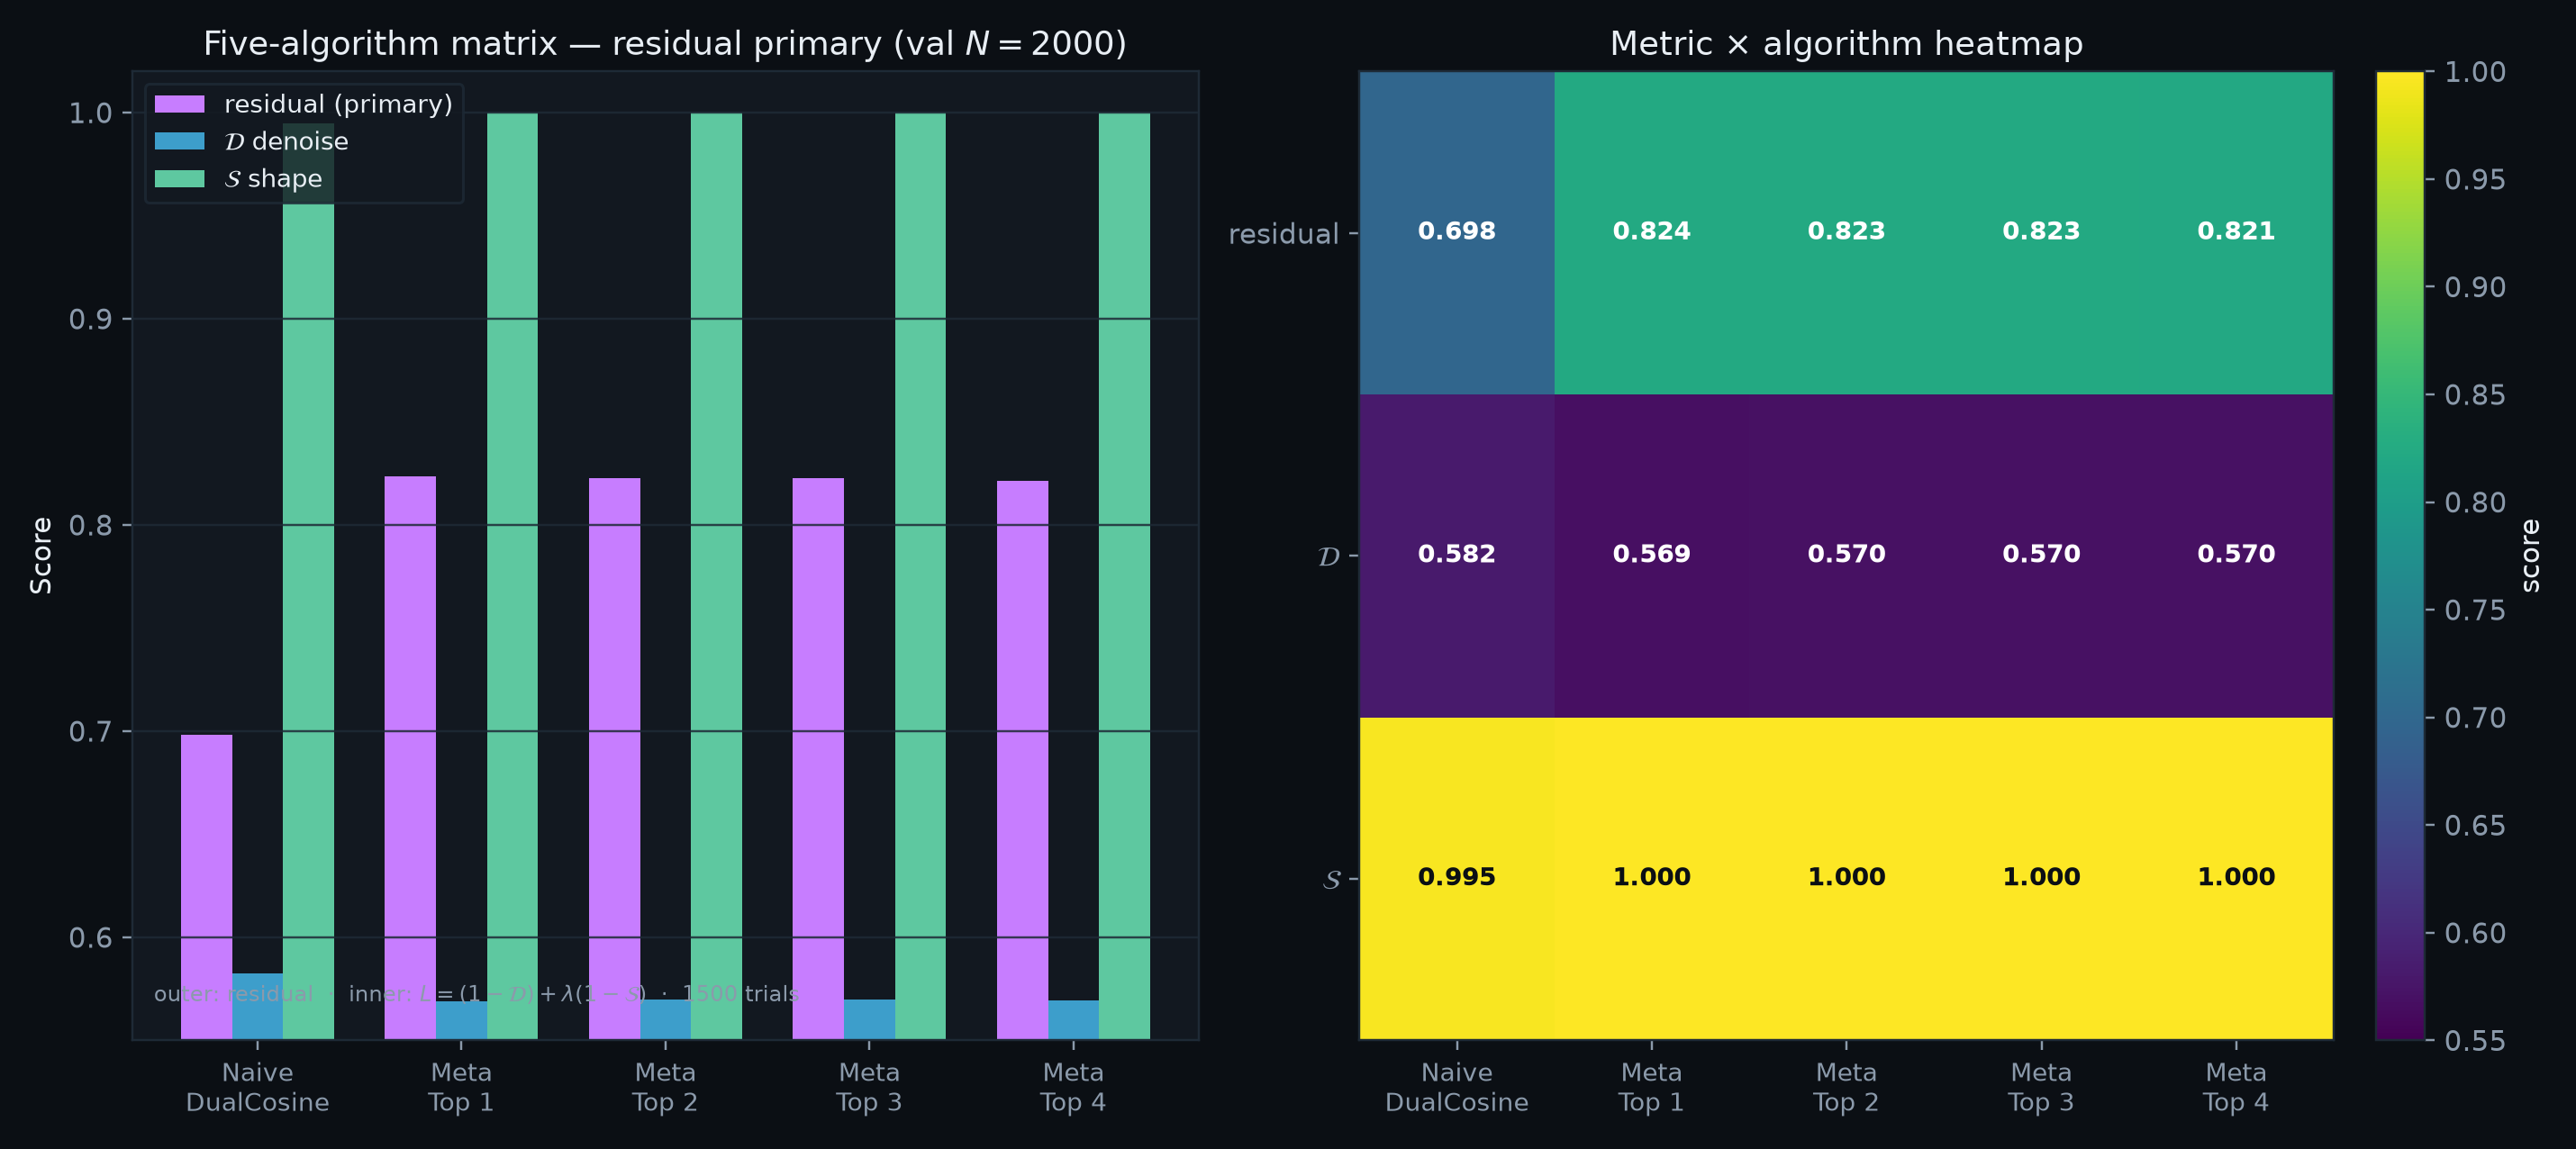
\includegraphics[width=0.88\textwidth]{figures/fig_benchmark_matrix.png}
  \caption{Naive DualCosine vs Meta Top 1--4 under residual (primary), denoise D, and shape S.}
  \label{fig:fig_benchmark_matrix}
\end{figure}

\begin{figure}[htbp]
  \centering
  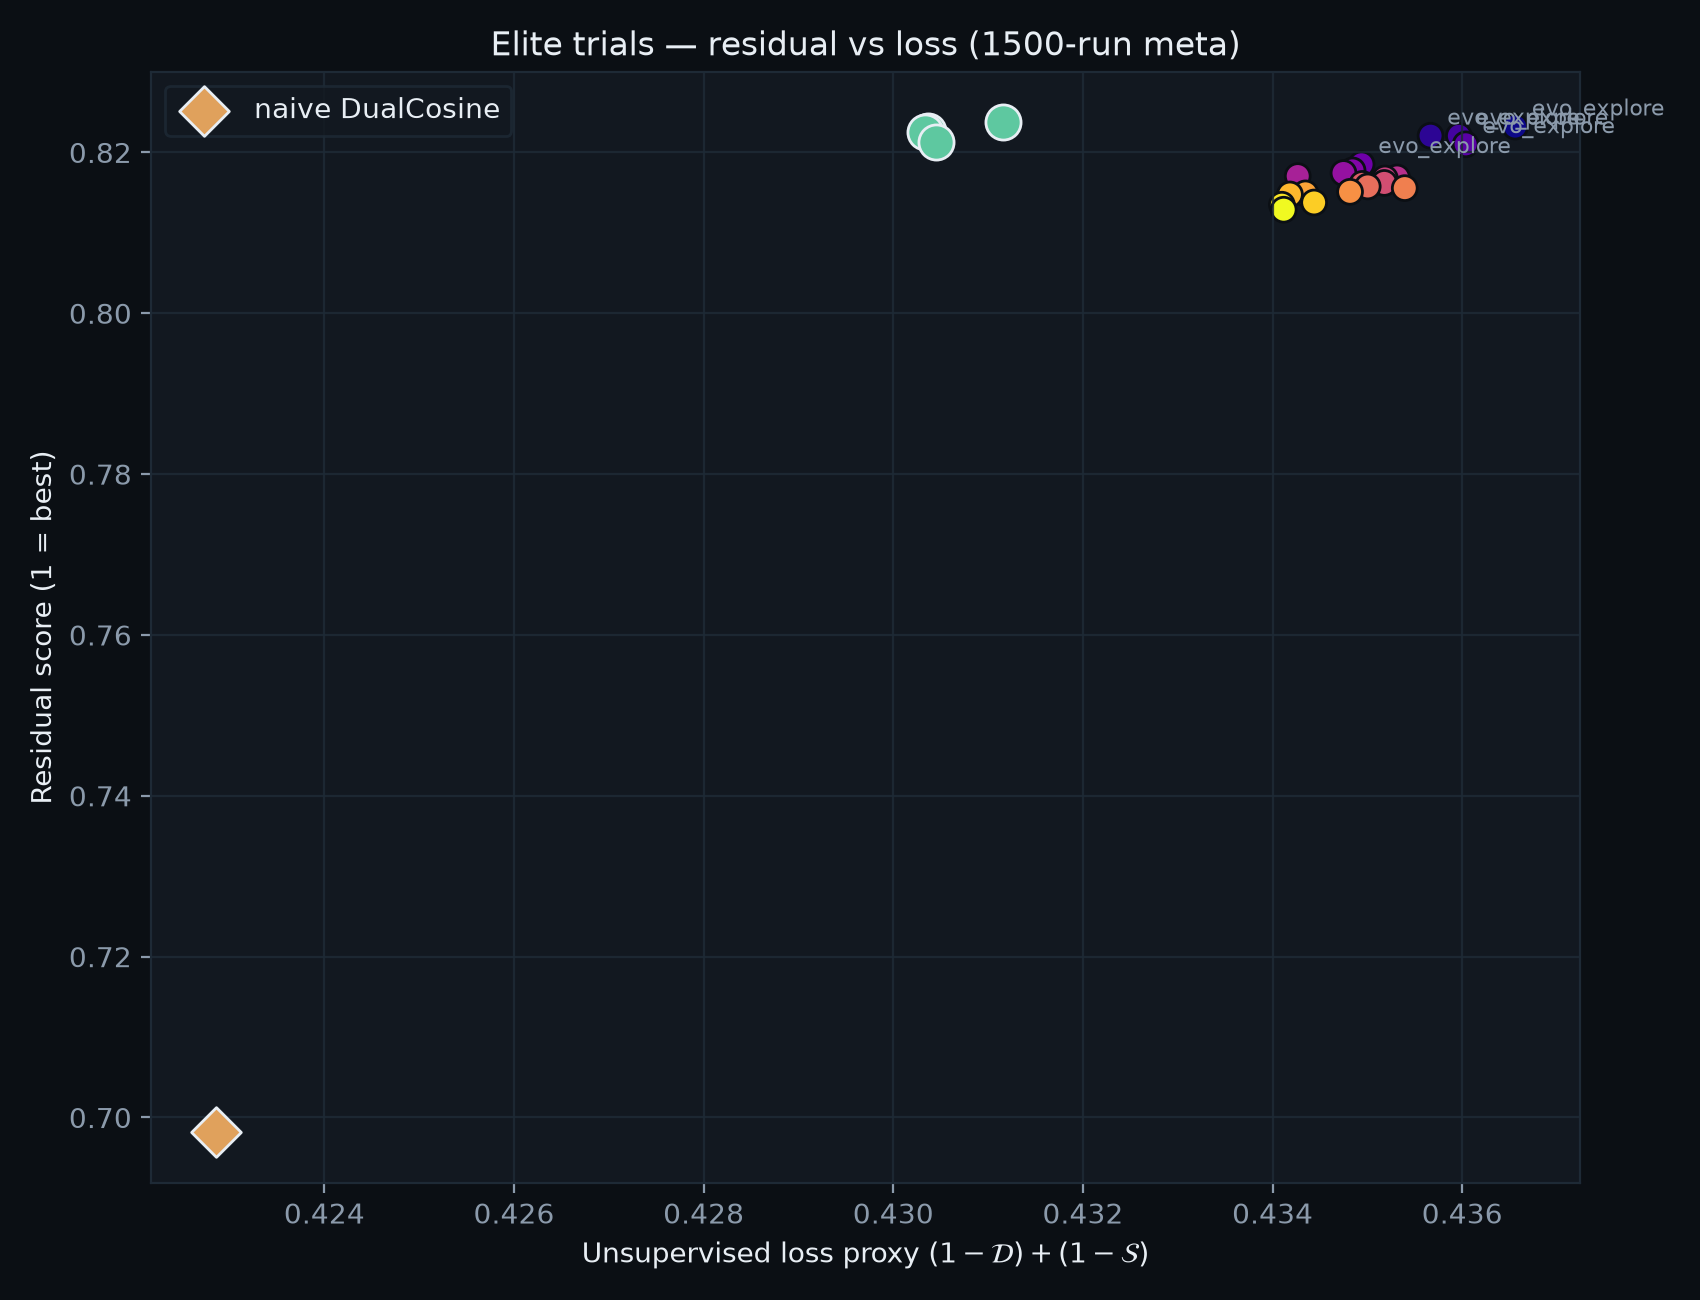
\includegraphics[width=0.88\textwidth]{figures/fig_pareto_1500.png}
  \caption{Elite residual versus unsupervised-loss proxy after 1500 trials.}
  \label{fig:fig_pareto_1500}
\end{figure}

\begin{figure}[htbp]
  \centering
  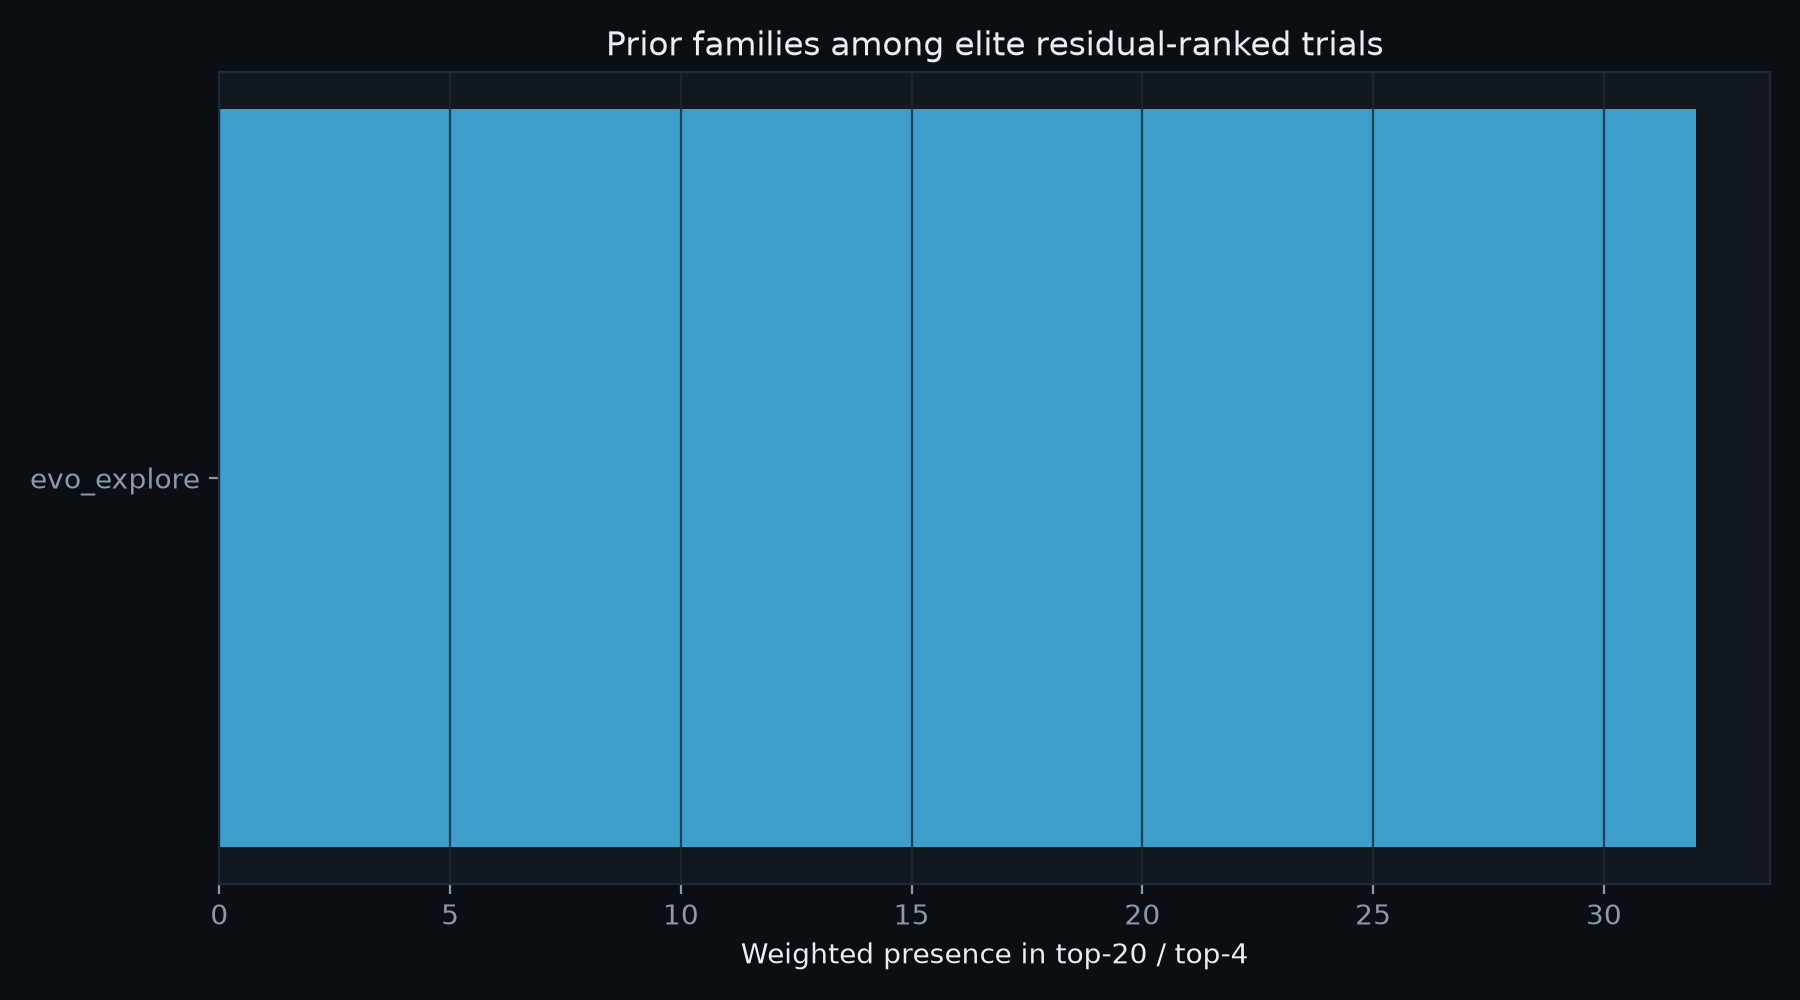
\includegraphics[width=0.88\textwidth]{figures/fig_prior_families.png}
  \caption{Prior families among residual elites (top-20 / top-4).}
  \label{fig:fig_prior_families}
\end{figure}

\paragraph{Honest note on nested loss optimization.}

All twenty Pareto-fast residual elites were evo\_explore (inner sweeps = 0). Bi-level / PBT / Bayes loss-opt priors were evaluated but did not win on residual. Inner L-minimization remains part of the search design as a nested regularizer; under prolonged residual, lighter evolutionary mutations currently dominate.

\section{Discussion}
Residual scoring shifts the outer objective from seam-local wrap energy toward agreement with prolonged cyclic playback against a known ideal tiling. Under that objective, the empirical killer configuration is \texttt{evo\_explore\_515}, arising from wide evolutionary mutation rather than the deepest nested loss fit.

This outcome is informative rather than anomalous: bi-level and related loss-opt priors were present in the search mixture and evaluated fairly; they did not dominate the residual elite set on this protocol. Inner $L$-minimization remains useful as a nested regularizer on D/S-shaped landscapes, but prolonged residual currently favors lighter mutate-only explore.

Practitioners should therefore treat residual as the deployment-facing score while retaining wrap-energy diagnostics as sanity checks for shape collapse.

\section{Limitations}
Validity threats include:
\begin{itemize}
  \item Residual uses a procedural ideal (no-cliff sibling), not a perceptual MOS.
  \item Bake metrics are not listening tests.
  \item Nested loss budgets are small (48 seeds) by design for 1500-trial throughput.
  \item Results are tied to the reported seed protocol and validation sizes.
\end{itemize}

\section{Conclusion}
We presented a prolonged residual objective for label-free wrap-crackle reduction and a literature-informed search over DenoiseOpt parameters. On the held-out matrix, \texttt{evo\_explore\_515} attains residual $0.8237$ versus DualCosine $0.6981$ ($\Delta\approx 0.1256$). Nested unsupervised loss optimization was searched and reported honestly; evolutionary explore dominated the residual elite set. Artifacts and frozen parameters are released with the companion repositories.

\begin{thebibliography}{99}

\bibitem{valimaki2006va} V. Valimaki, A. Huovilainen (2006). \emph{Oscillator and Filter Algorithms for Virtual Analog Synthesis}. Computer Music Journal, 30(2).

\bibitem{esqueda2016aliasing} F. Esqueda, S. Bilbao, V. Valimaki (2016). \emph{Aliasing Reduction in Clipped Signals}. IEEE Trans. Signal Processing.

\bibitem{esqueda2016blamp} F. Esqueda, V. Valimaki, S. Bilbao (2016). \emph{Rounding corners with BLAMP}. Proc. DAFx.

\bibitem{shan2021dwt} S. Shan et al. (2021). \emph{Differentiable Wavetable Synthesis}. arXiv:2111.10003.

\bibitem{lehtinen2018n2n} J. Lehtinen et al. (2018). \emph{Noise2Noise: Learning Image Restoration without Clean Data}. ICML.

\bibitem{snoek2012bo} J. Snoek, H. Larochelle, R. P. Adams (2012). \emph{Practical Bayesian Optimization of Machine Learning Algorithms}. NeurIPS.

\bibitem{bischl2023hpo} B. Bischl et al. (2023). \emph{Hyperparameter optimization: Foundations, algorithms, best practices}.

\bibitem{lopez2016irace} M. Lopez-Ibanez et al. (2016). \emph{The irace package: Iterated racing for automatic algorithm configuration}. Operations Research Perspectives.

\bibitem{zhang2007moead} Q. Zhang, H. Li (2007). \emph{MOEA/D: A Multiobjective Evolutionary Algorithm Based on Decomposition}. IEEE Trans. Evolutionary Computation.

\bibitem{finn2017maml} C. Finn, P. Abbeel, S. Levine (2017). \emph{Model-Agnostic Meta-Learning for Fast Adaptation of Deep Networks}. ICML. \textit{(Screened.)}

\end{thebibliography}
\end{document}
